\section{Faster Python and Glueing}

\subsection{Python as a glue}

\begin{frame}{Using Python as glue}

Python can wrap different different other programming languages\\[1ex]

\begin{exbox}{{\texttt{Cython}}}
    compiled, \emph{typed} Python - interface C/C++ code
\end{exbox}

\begin{exbox}{{\texttt{f2py}}}
    Fortran wrapper, included in NumPy
\end{exbox}

Why do that?
\begin{columns}

\column{0.5\textwidth}
\begin{itemize}
    \item Python can be \emph{slow}
    \item Python loops are slow
    \item calling Python functions is slow
\end{itemize}

\column{0.5\textwidth}
\begin{itemize}
    \item Wrap external C/Fortran... libraries
    \item Happily/unfortunately (?) there is legacy code
\end{itemize}

\end{columns}

\end{frame}


\subsection{A Problem}

\begin{frame}[fragile]{Problem: $\mathrm{sinc}(x)^{2}$}

\begin{Verbatim}[commandchars=\\\{\}]
\PY{k+kn}{import} \PY{n+nn}{numpy} \PY{k+kn}{as} \PY{n+nn}{np}
\PY{k+kn}{from} \PY{n+nn}{math} \PY{k+kn}{import} \PY{n}{sin}\PY{p}{,} \PY{n}{pi}

\PY{k}{def} \PY{n+nf}{sincSquare}\PY{p}{(}\PY{n}{x}\PY{p}{)}\PY{p}{:}
    \PY{l+s+sd}{"""Return the sinc(x) = (sin(x)/x)**2 of the array}
\PY{l+s+sd}{    argument x.}
\PY{l+s+sd}{    """}
    \PY{n}{retVal} \PY{o}{=} \PY{n}{np}\PY{o}{.}\PY{n}{zeros\PYZus{}like}\PY{p}{(}\PY{n}{x}\PY{p}{)}
    \PY{k}{for} \PY{n}{i} \PY{o+ow}{in} \PY{n+nb}{range}\PY{p}{(}\PY{n+nb}{len}\PY{p}{(}\PY{n}{x}\PY{p}{)}\PY{p}{)}\PY{p}{:}
        \PY{n}{retVal}\PY{p}{[}\PY{n}{i}\PY{p}{]} \PY{o}{=} \PY{p}{(}\PY{n}{sin}\PY{p}{(}\PY{n}{pi}\PY{o}{*}\PY{n}{x}\PY{p}{[}\PY{n}{i}\PY{p}{]}\PY{p}{)} \PY{o}{/} \PY{p}{(}\PY{n}{pi}\PY{o}{*}\PY{n}{x}\PY{p}{[}\PY{n}{i}\PY{p}{]}\PY{p}{)}\PY{p}{)}\PY{o}{*}\PY{o}{*}\PY{l+m+mi}{2}

    \PY{k}{return} \PY{n}{retVal}
\end{Verbatim}


\pause
$10^{6}$ array elements: {\texttt{1 loops, best of 3: 4.91 s per loop}}
\end{frame}


\begin{frame}{First attempt: use NumPy array operations}

\begin{Verbatim}[commandchars=\\\{\}]
\PY{k+kn}{import} \PY{n+nn}{numpy} \PY{k+kn}{as} \PY{n+nn}{np}

\PY{k}{def} \PY{n+nf}{sincSquareNumPy1}\PY{p}{(}\PY{n}{x}\PY{p}{)}\PY{p}{:}

    \PY{k}{return} \PY{p}{(}\PY{n}{np}\PY{o}{.}\PY{n}{sin}\PY{p}{(}\PY{n}{np}\PY{o}{.}\PY{n}{pi}\PY{o}{*}\PY{n}{x}\PY{p}{[}\PY{p}{:}\PY{p}{]}\PY{p}{)}\PY{o}{/}\PY{p}{(}\PY{n}{np}\PY{o}{.}\PY{n}{pi}\PY{o}{*}\PY{n}{x}\PY{p}{[}\PY{p}{:}\PY{p}{]}\PY{p}{)}\PY{p}{)}\PY{o}{*}\PY{o}{*}\PY{l+m+mi}{2}

\PY{k}{def} \PY{n+nf}{sincSquareNumPy2}\PY{p}{(}\PY{n}{x}\PY{p}{)}\PY{p}{:}

    \PY{k}{return} \PY{n}{np}\PY{o}{.}\PY{n}{sinc}\PY{p}{(}\PY{n}{x}\PY{p}{[}\PY{p}{:}\PY{p}{]}\PY{p}{)}\PY{o}{*}\PY{o}{*}\PY{l+m+mi}{2}
\end{Verbatim}


\pause
$10^{6}$ array elements: first function: {\texttt{10 loops, best of 3: 73 ms per loop}},
second function: {\texttt{10 loops, best of 3: 92.9 ms per loop}}

\end{frame}


\subsection{Cython by example}

\begin{frame}{How Cython works}

\begin{exbox}{Cython}
compiled, possibly typed Python:\\[1ex]
{\texttt{.pyx file}} $\stackrel{\text{Cython}}{\Longrightarrow}$ {\texttt{.c file}} $\stackrel{\text{C compiler}}{\Longrightarrow}$ {\texttt{.so/.dll file}}
\end{exbox}

\begin{itemize}
    \item various levels of typing possible
    \item C output and Cython's opinion on code speed can easily be
    inspected (optional {\texttt{.html}} output)
    \item interfacing C libraries is easy
\end{itemize}

\end{frame}


\begin{frame}[fragile]{$\mathrm{sinc}(x)^{2}$ - Cython, Version 1}

\begin{Verbatim}[commandchars=\\\{\}]
\PY{k}{cdef} \PY{k+kr}{extern} \PY{k}{from} \PY{l+s}{"}\PY{l+s}{math.h}\PY{l+s}{"}\PY{p}{:}
    \PY{n}{double} \PY{n}{sin}\PY{p}{(}\PY{n}{double}\PY{p}{)}
    \PY{n}{double} \PY{n+nb}{pow}\PY{p}{(}\PY{n}{double}\PY{p}{,} \PY{n+nb}{int}\PY{p}{)}

\PY{k}{def} \PY{n+nf}{sincSquareCython1}\PY{p}{(}\PY{n}{x}\PY{p}{)}\PY{p}{:}

    \PY{n}{pi} \PY{o}{=} \PY{l+m+mf}{3.1415926535897932384626433}
    \PY{n}{retVal} \PY{o}{=} \PY{n}{np}\PY{o}{.}\PY{n}{zeros\PYZus{}like}\PY{p}{(}\PY{n}{x}\PY{p}{)}

    \PY{k}{for} \PY{n}{i} \PY{o+ow}{in} \PY{n+nb}{range}\PY{p}{(}\PY{n+nb}{len}\PY{p}{(}\PY{n}{x}\PY{p}{)}\PY{p}{)}\PY{p}{:}
        \PY{n}{retVal}\PY{p}{[}\PY{n}{i}\PY{p}{]} \PY{o}{=} \PY{p}{(}\PY{n}{sin}\PY{p}{(}\PY{n}{pi}\PY{o}{*}\PY{n}{x}\PY{p}{[}\PY{n}{i}\PY{p}{]}\PY{p}{)} \PY{o}{/} \PY{p}{(}\PY{n}{pi}\PY{o}{*}\PY{n}{x}\PY{p}{[}\PY{n}{i}\PY{p}{]}\PY{p}{)}\PY{p}{)}\PY{o}{*}\PY{o}{*}\PY{l+m+mf}{2}

    \PY{k}{return} \PY{n}{retVal}
\end{Verbatim}


\pause
$10^{6}$ array elements: {\texttt{1 loops, best of 3: 4.39 s per loop}}
\end{frame}


\begin{frame}[fragile]{$\mathrm{sinc}(x)^{2}$ - Cython, Version 2}

\begin{Verbatim}[commandchars=\\\{\}]
\PY{k}{cimport} \PY{n+nn}{numpy} \PY{k}{as} \PY{n+nn}{np} \PY{c}{\PYZsh{} also C-import types}

\PY{k}{cpdef} \PY{k+kt}{np}.\PY{k+kt}{ndarray}[\PY{k+kt}{double}] \PY{k+kt}{sincSquareCython2}\PYZbs{}
    \PY{p}{(}\PY{n}{np}\PY{o}{.}\PY{n}{ndarray}\PY{p}{[}\PY{n}{double}\PY{p}{]} \PY{n}{x}\PY{p}{)}\PY{p}{:}

    \PY{k}{cdef} \PY{k+kt}{int} \PY{n+nf}{i}
    \PY{k}{cdef} \PY{k+kt}{double} \PY{n+nf}{pi} \PY{o}{=} \PY{l+m+mf}{3.1415926535897932384626433}
    \PY{k}{cdef} \PY{k+kt}{np}.\PY{k+kt}{ndarray}[\PY{k+kt}{double}] \PY{n+nf}{retVal} \PY{o}{=} \PY{n}{np}\PY{o}{.}\PY{n}{zeros\PYZus{}like}\PY{p}{(}\PY{n}{x}\PY{p}{)}

    \PY{k}{for} \PY{n}{i} \PY{o+ow}{in} \PY{n+nb}{range}\PY{p}{(}\PY{n+nb}{len}\PY{p}{(}\PY{n}{x}\PY{p}{)}\PY{p}{)}\PY{p}{:}
        \PY{n}{retVal}\PY{p}{[}\PY{n}{i}\PY{p}{]} \PY{o}{=} \PY{n+nb}{pow}\PY{p}{(}\PY{n}{sin}\PY{p}{(}\PY{n}{pi}\PY{o}{*}\PY{n}{x}\PY{p}{[}\PY{n}{i}\PY{p}{]}\PY{p}{)} \PY{o}{/} \PY{p}{(}\PY{n}{pi}\PY{o}{*}\PY{n}{x}\PY{p}{[}\PY{n}{i}\PY{p}{]}\PY{p}{)}\PY{p}{,} \PY{l+m+mf}{2}\PY{p}{)}
\end{Verbatim}


\pause
$10^{6}$ array elements: {\texttt{10 loops, best of 3: 49.1 ms per loop}}\\[0.5ex]
That's a \alert{speedup by a factor $\approx 100$}!
\end{frame}

\subsection{f2py by example}

\begin{frame}{How f2py works}

\begin{exbox}{f2py}
wrap Fortran code in Python:\\[1ex]
{\texttt{.f/.f90 file}} $\stackrel{\text{f2py}}{\Longrightarrow}$ {\texttt{.so/.dll file}}
\end{exbox}

\begin{itemize}
    \item f2py is included in NumPy
    \item exposes NumPy arrays to Fortran code
    \item once 'Fortran space' is entered, you run at full Fortran speed
\end{itemize}

\end{frame}


\begin{frame}[fragile]{$\mathrm{sinc}(x)^{2}$ - f2py, Version 1}

\begin{Verbatim}[commandchars=\\\{\}]
\PY{k}{subroutine }\PY{n+nv}{sincsquaref2py1}\PY{p}{(}\PY{n+nv}{x}\PY{p}{,} \PY{n+nv}{n}\PY{p}{,} \PY{n+nv}{outVal}\PY{p}{)}
    \PY{k}{implicit }\PY{k}{none}

\PY{k}{    }\PY{k+kt}{double precision}\PY{p}{,} \PY{k}{dimension}\PY{p}{(}\PY{n+nv}{n}\PY{p}{)}\PY{p}{,} \PY{k}{intent}\PY{p}{(}\PY{n+nv}{in}\PY{p}{)} \PY{k+kd}{::} \PY{n+nv}{x}
    \PY{k+kt}{integer}\PY{p}{,} \PY{k}{intent}\PY{p}{(}\PY{n+nv}{in}\PY{p}{)} \PY{k+kd}{::} \PY{n+nv}{n}
    \PY{k+kt}{double precision}\PY{p}{,} \PY{k}{dimension}\PY{p}{(}\PY{n+nv}{n}\PY{p}{)}\PY{p}{,} \PY{k}{intent}\PY{p}{(}\PY{n+nv}{out}\PY{p}{)} \PY{k+kd}{::} \PY{n+nv}{outVal}
    \PY{k+kt}{double precision}\PY{p}{,} \PY{k}{parameter} \PY{k+kd}{::} \PY{n+nv}{pi} \PY{o}{=} \PY{l+m+mf}{4.0}\PY{n+nv}{d0} \PY{o}{*} \PY{n+nb}{atan}\PY{p}{(}\PY{l+m+mf}{1.0}\PY{n+nv}{d0}\PY{p}{)}

    \PY{n+nv}{outVal}\PY{p}{(}\PY{p}{:}\PY{p}{)} \PY{o}{=} \PY{p}{(}\PY{n+nb}{sin}\PY{p}{(}\PY{n+nv}{pi}\PY{o}{*}\PY{n+nv}{x}\PY{p}{(}\PY{p}{:}\PY{p}{)}\PY{p}{)} \PY{o}{/} \PY{p}{(}\PY{n+nv}{pi}\PY{o}{*}\PY{n+nv}{x}\PY{p}{(}\PY{p}{:}\PY{p}{)}\PY{p}{)}\PY{p}{)}\PY{o}{**}\PY{l+m+mi}{2}

\PY{k}{end }\PY{k}{subroutine }\PY{n+nv}{sincsquaref2py1}
\end{Verbatim}


\pause
$10^{6}$ array elements: {\texttt{10 loops, best of 3: 47.4 ms per loop}}\\
Again, a \alert{speedup by a factor of $\approx 100$}!

\end{frame}


\begin{frame}[fragile]{Cheating: $\mathrm{sinc}(x)^{2}$ - f2py, Version 2 - OpenMP}

\begin{Verbatim}[commandchars=\\\{\}]
\PY{k}{subroutine }\PY{n+nv}{sincsquaref2py2}\PY{p}{(}\PY{n+nv}{x}\PY{p}{,} \PY{n+nv}{n}\PY{p}{,} \PY{n+nv}{outVal}\PY{p}{)}
    \PY{k}{implicit }\PY{k}{none}
\PY{k}{    }\PY{k+kt}{double precision}\PY{p}{,} \PY{k}{dimension}\PY{p}{(}\PY{n+nv}{n}\PY{p}{)}\PY{p}{,} \PY{k}{intent}\PY{p}{(}\PY{n+nv}{in}\PY{p}{)} \PY{k+kd}{::} \PY{n+nv}{x}
    \PY{k+kt}{integer}\PY{p}{,} \PY{k}{intent}\PY{p}{(}\PY{n+nv}{in}\PY{p}{)} \PY{k+kd}{::} \PY{n+nv}{n}
    \PY{k+kt}{double precision}\PY{p}{,} \PY{k}{dimension}\PY{p}{(}\PY{n+nv}{n}\PY{p}{)}\PY{p}{,} \PY{k}{intent}\PY{p}{(}\PY{n+nv}{out}\PY{p}{)} \PY{k+kd}{::} \PY{n+nv}{outVal}
    \PY{k+kt}{integer} \PY{k+kd}{::} \PY{n+nv}{i}
    \PY{k+kt}{double precision}\PY{p}{,} \PY{k}{parameter} \PY{k+kd}{::} \PY{n+nv}{pi} \PY{o}{=} \PY{l+m+mf}{4.0}\PY{n+nv}{d0} \PY{o}{*} \PY{n+nb}{atan}\PY{p}{(}\PY{l+m+mf}{1.0}\PY{n+nv}{d0}\PY{p}{)}
    \PY{c}{!\PYZdl{}OMP PARALLEL DO SHARED(x, outVal)}
    \PY{k}{do }\PY{n+nv}{i} \PY{o}{=} \PY{l+m+mi}{1}\PY{p}{,} \PY{n+nv}{n}
        \PY{n+nv}{outVal}\PY{p}{(}\PY{n+nv}{i}\PY{p}{)} \PY{o}{=} \PY{p}{(}\PY{n+nb}{sin}\PY{p}{(}\PY{n+nv}{pi}\PY{o}{*}\PY{n+nv}{x}\PY{p}{(}\PY{n+nv}{i}\PY{p}{)}\PY{p}{)} \PY{o}{/} \PY{p}{(}\PY{n+nv}{pi}\PY{o}{*}\PY{n+nv}{x}\PY{p}{(}\PY{n+nv}{i}\PY{p}{)}\PY{p}{)}\PY{p}{)}\PY{o}{**}\PY{l+m+mi}{2}
    \PY{k}{end }\PY{k}{do}
    \PY{c}{!\PYZdl{}OMP END PARALLEL DO}
\PY{k}{end }\PY{k}{subroutine }\PY{n+nv}{sincsquaref2py2}
\end{Verbatim}


\pause
$10^{6}$ array elements, 2 Threads: {\texttt{10 loops, best of 3: 33.5 ms per loop}}
\end{frame}


\begin{frame}{$\mathrm{sinc}(x)^{2}$ - Overview}

Benchmark for an Intel i7:

\begin{center}
    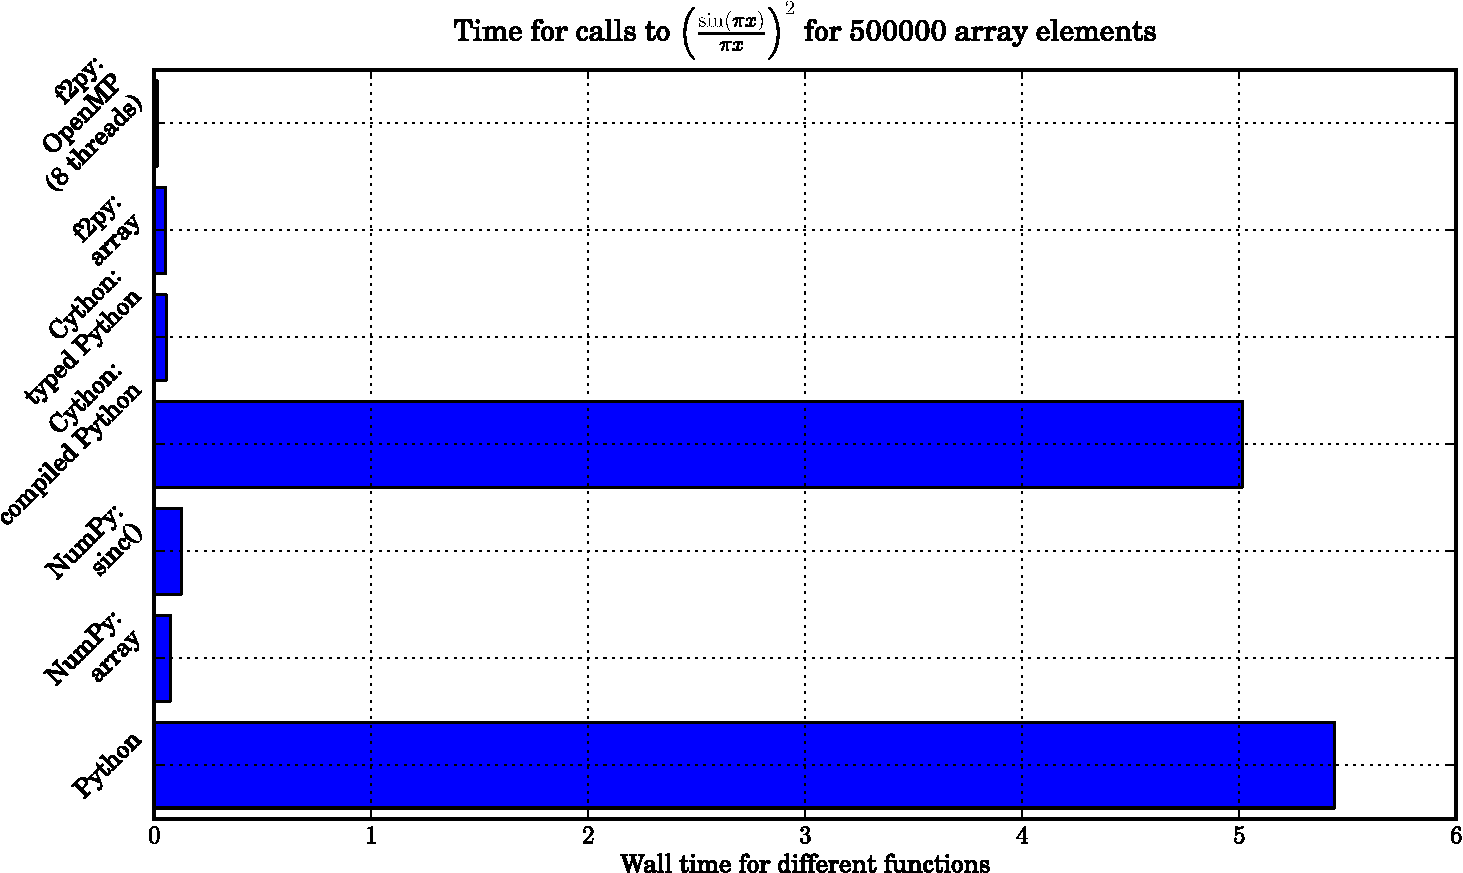
\includegraphics[width=1.0\textwidth]{Figures/benchmark}
\end{center}

\end{frame}


\subsection{Techniques for faster Scripts}

\begin{frame}{Techniques for faster Scripts}

After you have written a prototype in Python with NumPy and SciPy,
check if your code is already fast enough. If not,

\begin{itemize}
    \item profile your script (IPython's {\texttt{run -p}} or
    {\texttt{cProfile}} module...) to find bottlenecks
    \item if a large numbers of function calls is the bottleneck,
    typing and using  Cython's {\texttt{cdef/cpdef}} for C calling
    conventions speeds your code up at the cost of flexibility
    \item loops greatly benefit from typing, too
    \item consider moving heavy computations to Fortran/C completely -
    f2py and Cython will help you wrapping
\end{itemize}

\end{frame}


\subsection{MPI in Python}

\begin{frame}{Slightly OffTopic: mpi4py}

\begin{exbox}{mpi4py}
    Interface MPI in Python
\end{exbox}

\begin{itemize}
    \item speed-up pure Python by parallelization using MPI (OpenMPI, mpich...)
    \item mpi4py also works with f2py and Cython (?)
    \item[$\rightarrow$] run the steering Python script with
    {\texttt{mpirun...}}, take care of the communicator there and use
    it in Fortran, too
\end{itemize}

Alternatives:

\begin{itemize}
    \item IPython's parallel computing facilities
\end{itemize}

\end{frame}


\begin{frame}[fragile]{Slightly OffTopic: mpi4py}

\begin{Verbatim}[commandchars=\\\{\}]
\PY{k+kn}{from} \PY{n+nn}{mpi4py} \PY{k+kn}{import} \PY{n}{MPI}

\PY{n}{MPIroot} \PY{o}{=} \PY{l+m+mi}{0} \PY{c}{\PYZsh{} define the root process}
\PY{n}{MPIcomm} \PY{o}{=} \PY{n}{MPI}\PY{o}{.}\PY{n}{COMM\PYZus{}WORLD} \PY{c}{\PYZsh{} MPI communicator}

\PY{n}{MPIrank}\PY{p}{,} \PY{n}{MPIsize} \PY{o}{=} \PY{n}{MPIcomm}\PY{o}{.}\PY{n}{Get\PYZus{}rank}\PY{p}{(}\PY{p}{)}\PY{p}{,} \PY{n}{MPIcomm}\PY{o}{.}\PY{n}{Get\PYZus{}size}\PY{p}{(}\PY{p}{)}

\PY{o}{.}\PY{o}{.}\PY{o}{.}

\PY{n}{MPIcomm}\PY{o}{.}\PY{n}{Reduce}\PY{p}{(}\PY{n}{tempVals}\PY{p}{,} \PY{n}{retVal}\PY{p}{,} \PY{n}{op}\PY{o}{=}\PY{n}{MPI}\PY{o}{.}\PY{n}{SUM}\PY{p}{,} \PY{n}{root}\PY{o}{=}\PY{n}{MPIroot}\PY{p}{)}
\end{Verbatim}


\end{frame}
